\documentclass[12pt]{article}
\usepackage{amsmath}
\usepackage{graphicx}
\begin{document}
\title{Computer Science M151B, Homework 4}
\date{April 30th, 2018}
\author{Michael Wu\\UID: 404751542}
\maketitle

\section*{Problem 1}

\paragraph{a)}

The first program has
\[\frac{1.1 \text{ s} \times\frac{1 \text{ cycle}}{10^{-9} \text{ s}}}{10^9\text{ instructions}}\approx 1.1 \text{ CPI}\]
and the second has
\[\frac{1.5 \text{ s} \times\frac{1 \text{ cycle}}{10^{-9} \text{ s}}}{1.2\times 10^9\text{ instructions}}\approx 1.25 \text{ CPI}\]

\paragraph{b)}

Changing the processor means that both the cycles per instruction could change and the clock speed could change, so we cannot make any conclusions
about the relative clock speeds of the different processors.

\paragraph{c)}

The new compiler will generate an executable with the execution time
\[\frac{6\times 10^8 \text{ instructions} \times 1.1 \text{ CPI}}{10^9 \text{ cycles/s}} = 0.66 \text{ s}\]
which represents a
\[\frac{1.1\text{ s}}{0.66\text{ s}}\approx 1.667\]
times speedup over compiler A's program, and a
\[\frac{1.5\text{ s}}{0.66\text{ s}}\approx 2.273\]
times speedup over compiler B's program.

\section*{Problem 2}

\begin{align*}
        \frac{1}{10.1}&=\frac{1}{x}\times\frac{1}{2.45}\\
        x&=\frac{10.1}{2.45}\\
        x&\approx 4.122
\end{align*}
The programmer's instruction count is improved by a factor of approximately \(4.122\) relative to the compiler's.

\section*{Problem 3}

We need to find the total number of cycles over the total number of instructions.
Let \(r\) be the clock rate in cycles per second. Then the total number of instructions \(i\) is given by
\[i=r\left(\frac{3.8\text{ s}}{3\text{ CPI}}+\frac{8.5\text{ s}}{3.5\text{ CPI}}\right)=r\frac{388}{105}\text{ instructions}\]
and the total number of cycles \(c\) is given by
\[c=r(3.8\text{ s}+8.5\text{ s})=r\frac{123}{10}\text{ cycles}\]
Then we have that the new cycles per instruction will be
\[\frac{r\frac{123}{10}\text{ cycles}}{r\frac{388}{105}\text{ instructions}}\approx 3.329 \text{ CPI}\]

\section*{Problem 4}

\paragraph{a)}

Let \(i\) be the number of instructions in the program. The cycles per instruction \(x\) of non floating point operations is given by
\begin{align*}
        \frac{0.82i\times x+0.18i\times 5.3\text{ CPI}}{i}&=3.6\text{ CPI}\\
        x&\approx 3.227 \text{ CPI}
\end{align*}
Then the overall cycles per instruction for the improved processor is
\[\frac{0.82i\times 3.227\text{ CPI}+0.18i\times 3\text{ CPI}}{i} \approx 3.186\text{ CPI}\]

\paragraph{b)}

It would take \(194.7\text{ s}\) to execute the program on the improved processor.

\section*{Problem 5}

\paragraph{a)}

I would add an instruction memory unit so that the final step of load and store can be done in parallel with the instruction fetch. The last
state of both the load and store instructions would point to the instruction decode step, reducing the cycles per instruction by 1.

\begin{figure}[!ht]
    \begin{center}
        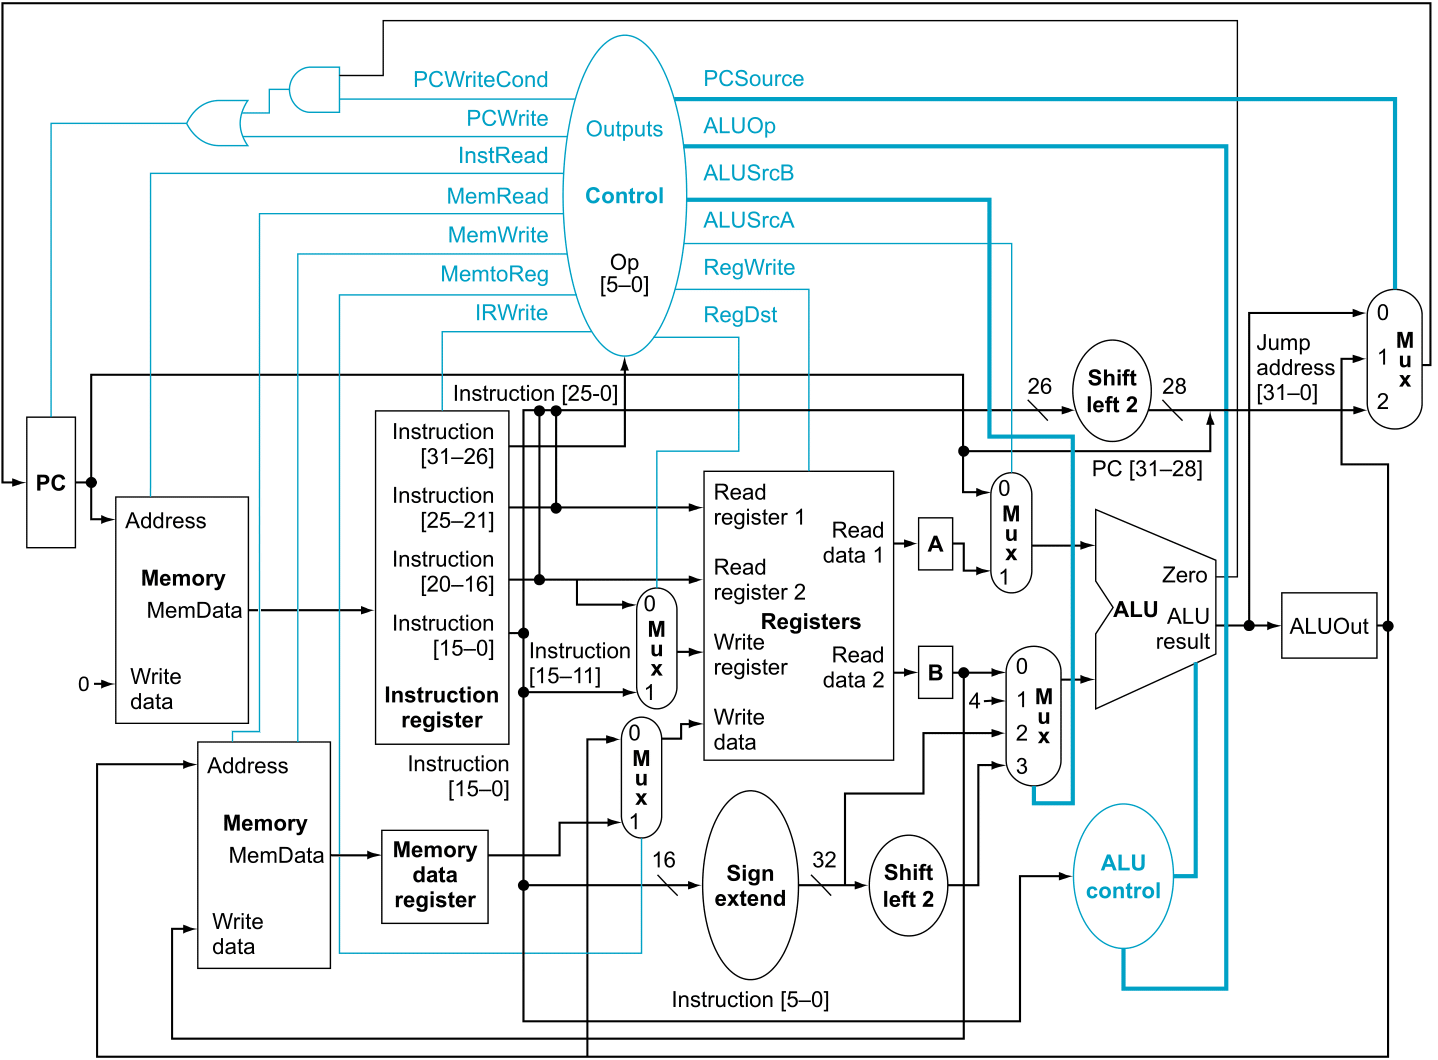
\includegraphics[width=4.8in]{problem5b.png}
    \end{center}
\end{figure}

\paragraph{b)}

The datapath changes above show the addition of the instruction memory unit. I input a zero to the \texttt{write data} signal of the instruction memory
unit since it should not be doing any writing, so this value will never be used.

\paragraph{c)}

The control signal \texttt{IorD} is renamed to \texttt{InstRead}, since there is no need for a multiplexer to choose between reading instruction memory or
regular memory. This signal controls whether to read from the address stored in the program counter or not.

\begin{figure}[!ht]
    \begin{center}
        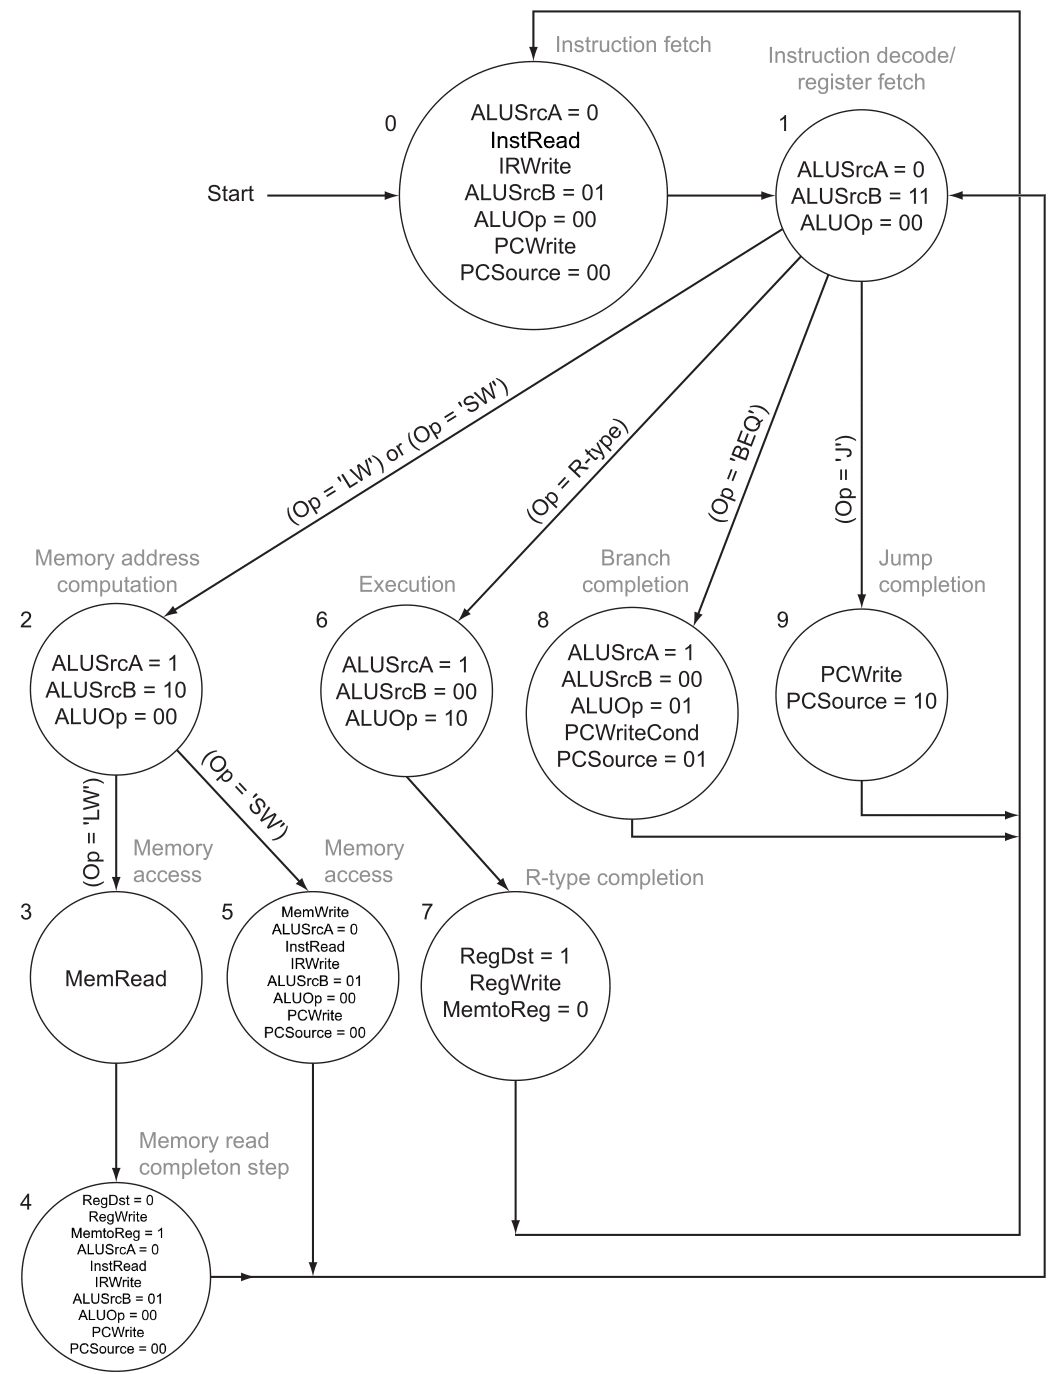
\includegraphics[width=4.7in]{problem5d.png}
    \end{center}
\end{figure}

\paragraph{d)}

The state changes are shown above. I have removed \texttt{IorD} and have allowed for the instruction fetch to happen at the same time as the last states
of the load and store instructions. This allows them to immediately go to the instruction decode step, reducing the number of cycles required by 1.

\section*{Problem 6}

Since \texttt{lw} uses every stage of the pipeline, its latency will be \(1750\text{ ps}\) in the pipelined processor. This is because the clock cycle
in a pipelined processor will be equivalent to the latency of the longest stage, which is \(350\text{ ps}\). So \texttt{lw} will execute over \(5\) clock
cycles. In the equivalent non-pipelined processor that uses a single cycle implementation, the clock cycle must accommodate the longest instruction.
This would mean that the clock cycle length is the sum of all the latencies of the instruction stages, and so it would be \(1250\text{ ps}\). So in
the non-pipelined processor \texttt{lw} would have a latency of \(1250\text{ ps}\).

\section*{Problem 7}

I would split the \texttt{ID} stage of the pipelined datapath into two, as this will decrease the latency of the longest stage to \(300\text{ ps}\). So
the new clock cycle time of the processor would be \(300\text{ ps}\).

\section*{Problem 8}

The instruction \(i_1\)
\begin{verbatim}
or r1, r2, r3
\end{verbatim}
has no data dependencies. The instruction \(i_2\)
\begin{verbatim}
or r2, r1, r4
\end{verbatim}
has a data dependency on the first instruction \(i_1\). There is a Read After Write (RAW) data dependency, and it occurs due to \(i_1\) writing to
\texttt{r1} before \(i_2\) reads from \texttt{r1}. There is also a Write After Read (WAR) dependency due to \(i_1\) reading from \texttt{r2} before
\(i_2\) writes to \texttt{r2}.
The instruction \(i_3\)
\begin{verbatim}
or r1, r1, r2
\end{verbatim}
has data dependencies on both \(i_1\) and \(i_2\). There is a RAW dependency due to \(i_i\) writing to \texttt{r1} before \(i_3\) reads from \texttt{r1}.
There is a Write After Write (WAW) dependency due to \(i_1\) writing to \texttt{r1} before \(i_3\) writes to \texttt{r1}. There is a RAW dependency due to
\(i_2\) writing to \texttt{r2} before \(i_3\) reads from \texttt{r2}. Finally, there is a WAR dependency due to \(i_2\) reading from \texttt{r1} before \(i_3\)
writes to \texttt{r1}. Note that in our simple pipelined processor we only really need to be concerned about RAW dependencies, since we do not do out-of-order
execution. So WAR and WAW dependencies will be taken care of and not change the execution in any way.

\section*{Problem 9}

I will use
\begin{verbatim}
add $zero, $zero, $zero
\end{verbatim}
as my \texttt{nop}. Then we need to ensure that all dependencies are taken care of. As noted before, WAR and WAW will be taken care of already because our processor
does not do out of order execution. They are not a hazard, but the RAW dependencies represent a data hazard. To ensure that the RAW dependencies are taken care of,
we must ensure that the \texttt{ID} stage of an instruction occurs after the \texttt{WB} stage of the previous instruction. This means that we need three
\texttt{nop} instructions between each original instruction, because \texttt{WB} is the fifth stage and \texttt{ID} is the second stage. So our final program
will be the code shown below.
\begin{verbatim}
or  r1,    r2,    r3
add $zero, $zero, $zero
add $zero, $zero, $zero
add $zero, $zero, $zero
or  r2,    r1,    r4
add $zero, $zero, $zero
add $zero, $zero, $zero
add $zero, $zero, $zero
or  r1,    r1,    r2
\end{verbatim}

\section*{Problem 10}

As before, data hazards occur due to the RAW dependencies. But with full forwarding, they should not slow down execution and no \texttt{nop} instructions are
required. The instruction \(i_2\) will receive its ALU input through forwarding the contents of the \texttt{EX/MEM} register from \(i_1\), and the instruction
\(i_3\) will receive its ALU input through forwarding the contents of the \texttt{EX/MEM} register from \(i_2\) and the contents of the \texttt{MEM/WB} register from
\(i_1\).

\section*{Problem 11}

\paragraph{a)}

For the \texttt{sw} instruction, no control signals need to be asserted for the \texttt{IF} and \texttt{ID} stages. During the \texttt{EX} stage, the signals
\texttt{ALUOp = 00} and \texttt{ALUSrc = 1} are asserted. In this stage \texttt{MemWrite} is asserted, but it does not do anything and is passed along to the
next stage of execution. In the \texttt{MEM} stage, the signal \texttt{MemWrite} is asserted and performs the writing of data to memory. In the \texttt{WB} stage,
no control signals are asserted.

\paragraph{b)}

For the \texttt{sub} instruction, no control signals need to be asserted for the \texttt{IF} and \texttt{ID} stages. During the \texttt{EX} stage, the signals
\texttt{RegDst = 1}, \texttt{ALUOp = 10}, and \texttt{ALUSrc = 0} are asserted. In this stage \texttt{RegWrite} and \texttt{MemtoReg = 0} are asserted, but they
not do anything and are passed along to the next stage of execution. In the \texttt{MEM} stage, again \texttt{RegWrite} and \texttt{MemtoReg = 0} are asserted,
but they do not do anything and are passed along to the next stage of execution. In the \texttt{WB} stage, the signals \texttt{RegWrite} and \texttt{MemtoReg = 0}
are asserted, storing the results of the ALU operation into a register.

\end{document}